\section{\MakeUppercase {The Enactment-Scope Framework}}
\label{sec:Enactment-Scope}
\renewcommand{\baselinestretch}{2.0}\normalsize

\subsection{Three lines of work, one missing synthesis}

Resilience research has matured along three distinguishable but partial lines, and naming the differences between them clarifies what an integrative framework still has to do. 

The first line examines digital infrastructures and technological systems---how architectures, redundancy mechanisms, and reconfiguration capacities sustain services during disturbance. One strand gives empirically grounded accounts of detection, response, and recovery: \textcite{linkov2013resilience} propose a resilience matrix that scores cyber systems across plan, absorb, recover, and adapt stages; \textcite{bjorck2015cyber} fix the conceptual fundamentals of a cyber-resilience definition; \textcite{dupont2019cyberresilience} examines its significance and applicability in financial institutions; \textcite{hausken2020cyber} synthesizes cyber resilience across firms, organizations, and societies; and \textcite{kuypers2018designing} turn organizational incident data into design guidance for security operations---building on a longer IS tradition of security-risk planning \autocite{straub1998coping}. A second strand applies network analysis: \textcite{albert2000error} show that scale-free topologies tolerate random failures yet are fragile to targeted attack; \textcite{gao2016universal} reduce high-dimensional network dynamics to a universal resilience function; and \textcite{panteli2017metrics} operationalize infrastructure-resilience metrics for power systems. A third develops formal models of attack--defense dynamics: \textcite{zhu2015game} use game-theoretic, games-in-games methods to quantify resilient control of cyber-physical systems under adversarial pressure. Across these strands the work treats organizations primarily as operators of technical systems. 

The second line approaches resilience as an organizational capability, foregrounding leadership, mindfulness, governance, and learning routines. \textcite{weick2011managing} locate it in the mindful organizing of high-reliability organizations---preoccupation with failure, reluctance to simplify, sensitivity to operations, commitment to resilience, and deference to expertise---and \textcite{vogus2007organizational} sketch a corresponding theory and research agenda that casts resilience as positive adjustment sustained under strain. A capability-oriented strand then specifies the underlying mechanisms: \textcite{teece2007explicating} decomposes dynamic capabilities into sensing, seizing, and reconfiguring, with explicit microfoundations; \textcite{lengnick2011developing} trace how strategic human-resource practices build a latent \emph{capacity} for resilience across cognitive, behavioral, and contextual dimensions; \textcite{duchek2019organizational} recasts the construct as a process of anticipation, coping, and adaptation; and \textcite{bhamra2011resilience} consolidate the cross-disciplinary literature into a multi-level account. Most recently, \textcite{boh2023building} show how digital technologies and data underpin organizational resilience to major shocks. Collectively this line offers detailed accounts of internal resilience mechanisms but is lighter on the infrastructures through which those mechanisms now operate. 

The third line addresses the ecosystem level, where adaptive capacity is produced through coordination across organizational boundaries. One thread concerns interorganizational information flows: \textcite{arnold2004informationsharing} examine information-sharing in out-of-hospital disaster response and the enabling role of IT; \textcite{malhotra2005absorptive} show how absorptive-capacity configurations let supply-chain partners jointly create market knowledge; and \textcite{rai2006firm} link digitally enabled supply-chain integration capabilities to firm performance. A second thread concerns the platforms and networks through which such coordination runs: \textcite{tiwana2010research} model platform evolution as the coevolution of architecture, governance, and environmental dynamics; \textcite{janssen2006network} bring a network perspective to resilience in social-ecological systems; and \textcite{liu2022network} formalize how network structure governs resilience. A third concerns collective cyber defense specifically: \textcite{enisa2017isacs} document cooperative ISAC models for security information sharing, and \textcite{lostri2022shared} frame cybersecurity as a public--private shared responsibility. This line captures coordinated action across organizational boundaries but does less to connect ecosystem-level dynamics back to internal mechanisms.\\

Each line is strongest precisely where the others are thin, yet none specifies how its mechanisms depend on those the other two study---reproducing in research architecture the same misalignment that field interviews report in practice, where cross-unit coordination breaks down, compliance substitutes for adaptation, and exercises rarely change operational routines \autocite{rota2024}. Closing that gap requires more than another definition or a single-domain maturity model; it requires a framework that specifies how the three sets of mechanisms interlock across a socio-technical organization.\\

The Enactment--Scope framework is designed to provide that specification. Its \emph{enactment} dimension distinguishes three mechanisms through which resilience is realized---technological, managerial, and collaborative---mapping directly onto the three partial literatures above. Its \emph{scope} dimension locates those mechanisms across infrastructural, organizational, and ecosystem coordination boundaries. Crossing the two dimensions yields a 3$\times$3 grid that asks not only whether a resilience initiative exists, but whether mechanisms in one cell are supported or undermined by dependencies in others. That structure explains a recurring practical failure mode: initiatives that appear strong in isolation---mature SOC operations, cloud redundancy, Information Sharing and Analysis Center (ISAC) membership---still produce weak adaptive performance when the coupled cells remain thin, not least because security information sharing depends on behavioral participation that often remains reluctant even among ISAC members \autocite{skopik2016problem,mermoud2019share}.\\

The framework separates two tasks that policy and practice often conflate. The first is \emph{translation}: turning articulated resilience---strategy language, audit artifacts, board reporting---into capability that can actually be observed when disruption hits. Translation works as a closed loop rather than a checklist (Figure~\ref{fig:triangle}). Take a board commitment to restore a critical service within a fixed impact tolerance: on its own it is a sentence in a policy document, and it becomes capability only when three mechanisms engage in turn. \emph{Design principles} act first, allocating the decision rights and escalation paths that let an operator invoke failover without waiting for sign-off, so the intended response is structurally possible rather than blocked by hierarchy \autocite{boin2013resilient,nist2024csf}. \emph{Operational indicators} act next, logging who acted, how quickly reconfiguration occurred, and where coordination stalled---so adaptive performance leaves a measurable trace instead of a claim \autocite{watson2010information,linkov2013resilience}. \emph{Benchmarks and warning systems} act last, comparing that trace against the stated tolerance, flagging departure, and feeding the gap back into the next round of decisions and investment \autocite{bcbs2021operational}. Structure the action, observe it, correct it: run together the three close a loop that converts a declared intention into a capability that can be seen, judged, and improved---omit any one and resilience reverts to words. The second task is \emph{placement}: deciding where that loop, and the technological, managerial, and collaborative practices it governs, must sit in the socio-technical settings where organizations actually coordinate. Figure~\ref{fig:enactment_scope} (introduced below) maps concrete practices into the enactment--scope grid. Together the two figures specify what must be translated and where translation must land if resilience is to become governable and revisable as conditions evolve, rather than merely declarative.\\

\begin{figure}[t]
    \centering
    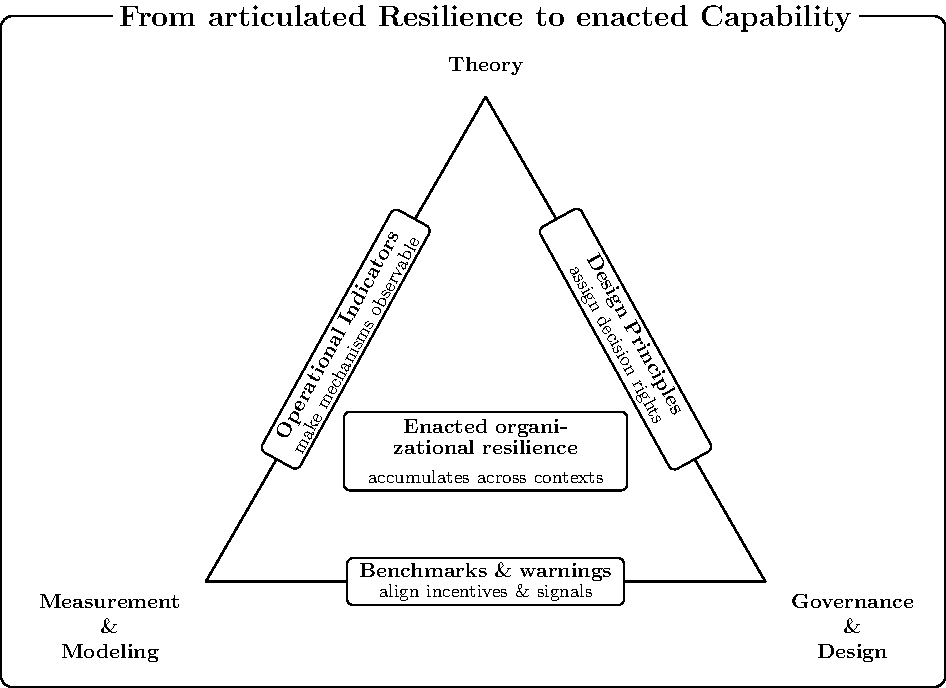
\includegraphics[width=0.8\linewidth]{figures_and_tables/Tikz_State_of_the_Art.pdf}
    \caption{\textbf{From articulated resilience to enacted capability.} Operational indicators make adaptive mechanisms observable. Design principles structure decision rights and coordination. Benchmarks and warning systems align incentives and signal deviation from desired states. Together, these mechanisms help translate resilience from a stated organizational commitment into enacted capability.}
    \label{fig:triangle}
\end{figure}

\subsection{Integrating Enactment and Scope}

\begin{figure}[!ht]
\centering
\small
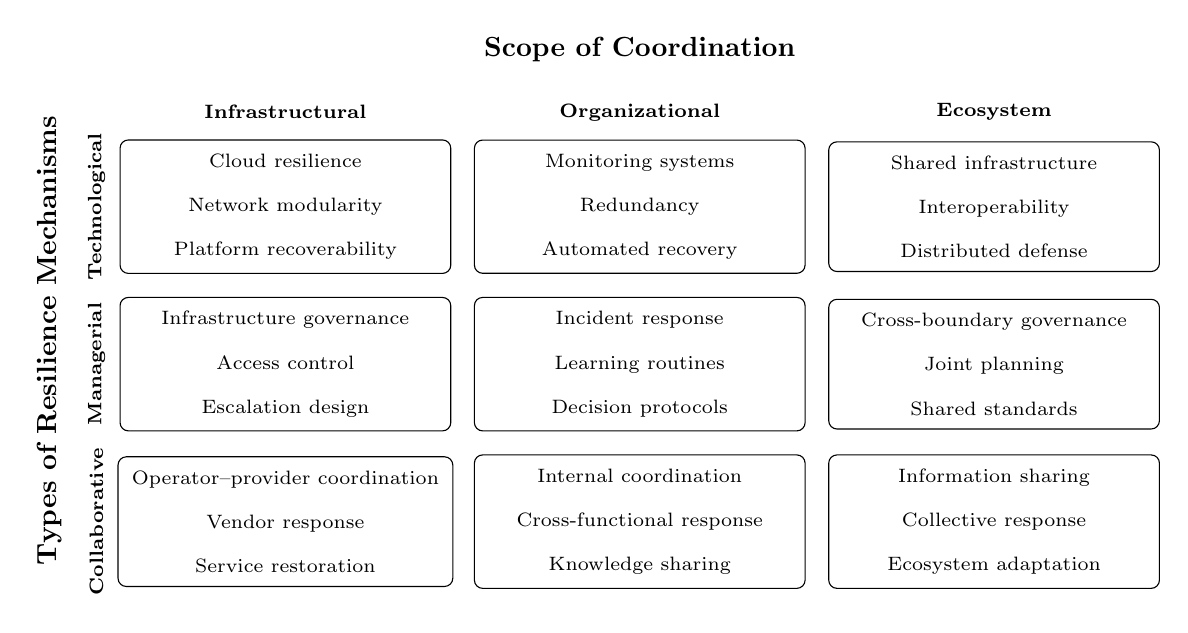
\begin{tikzpicture}[
    font=\small,
    cell/.style={
        draw,
        rounded corners=3pt,
        align=center,
        minimum width=4.2cm,
        minimum height=1.5cm,
        inner sep=5pt
    }
]

\node[font=\bfseries] at (6.5,4) {Scope of Coordination};
\node[rotate=90,font=\bfseries] at (-1,0.3) {Types of Resilience Mechanisms};

% Column titles
\node[font=\scriptsize] at (2,3.2) {\bfseries Infrastructural};
\node[font=\scriptsize] at (6.5,3.2) {\bfseries Organizational};
\node[font=\scriptsize] at (11,3.2) {\bfseries Ecosystem};

\node[rotate=90,font=\scriptsize] at (-0.4,2) {\bfseries Technological};
\node[rotate=90,font=\scriptsize] at (-0.4,0) {\bfseries Managerial};
\node[rotate=90,font=\scriptsize] at (-0.4,-2) {\bfseries Collaborative};

% Row 1
\node[cell,font=\scriptsize] at (2,2) {Cloud resilience\\Network modularity\\Platform recoverability};

\node[cell,font=\scriptsize] at (6.5,2) {Monitoring systems\\Redundancy\\Automated recovery};

\node[cell,font=\scriptsize] at (11,2) {Shared infrastructure\\Interoperability\\Distributed defense};

% Row 2
\node[cell,font=\scriptsize] at (2,0) {Infrastructure governance\\Access control\\Escalation design};

\node[cell,font=\scriptsize] at (6.5,0) {Incident response\\Learning routines\\Decision protocols};

\node[cell,font=\scriptsize] at (11,0) {Cross-boundary governance\\Joint planning\\Shared standards};

% Row 3
\node[cell,font=\scriptsize] at (2,-2) {Operator--provider coordination\\Vendor response\\Service restoration};

\node[cell,font=\scriptsize] at (6.5,-2) {Internal coordination\\Cross-functional response\\Knowledge sharing};

\node[cell,font=\scriptsize] at (11,-2) {Information sharing\\Collective response\\Ecosystem adaptation};

\end{tikzpicture}

\caption{\textbf{The Enactment–Scope Framework of Digital Organizational Resilience.}
Resilience mechanisms are enacted through technological, managerial, and collaborative processes, and operate across different scopes of coordination including infrastructural, organizational, and ecosystem levels.}
\label{fig:enactment_scope}
\end{figure}

Figure~\ref{fig:enactment_scope} renders the framework as a 3$\times$3 grid that locates concrete resilience mechanisms at their socio-technical address. Field interviews illustrate the coupling problem the grid is meant to expose: even within the organizational scope, IT, risk, and compliance units often operate in silos that constrain how internal mechanisms combine, let alone link to infrastructural and ecosystem-level coordination (Appendix~\ref{appendix:C}). Reading the grid by rows clarifies what each enactment mechanism contributes at each scope.\\

\emph{Technological} mechanisms operate through digital safeguards. At the infrastructural scope they are network-level properties---cloud resilience, modularity, platform recoverability---where scale-free fragility to targeted attack \autocite{albert2000error} and universal recovery dynamics \autocite{gao2016universal,panteli2017metrics} bound the design space. Inside the firm the same logic becomes a portfolio problem: \textcite{cavusoglu2009configuration} show that firewalls and intrusion-detection systems interact, so monitoring and automated recovery must be configured jointly rather than procured piecemeal, while \textcite{angst2017when} find that such investments reduce breaches only when substantively assimilated rather than symbolically adopted---redundancy and monitoring yield resilience only once genuinely embedded \autocite{linkov2013resilience,bjorck2015cyber,kuypers2018designing}. At the ecosystem scope the unit of analysis shifts to shared infrastructure, interoperability, and distributed defense \autocite{dupont2019cyberresilience,lostri2022shared}.\\

\emph{Managerial} mechanisms operate through human decision processes. At the infrastructural scope they govern access, escalation, and critical updates, codified in continuity and control standards \autocite{boin2013resilient,calder2021iso,nist2024csf}. Inside the firm they are the routines of incident response and learning---routines that, when an incident is declared, transiently reallocate decision authority toward those closest to the problem before handing it back, a shift Section~\ref{sec:RD} treats as a governed object in its own right---and the IS evidence is pointed about what makes them work: protective behavior follows from awareness of countermeasures and deterrence \autocite{darcy2009user}, from rationality-based beliefs and security awareness rather than mandate alone \autocite{anderson2010practicing,bulgurcu2010information}, and is sustained by the mindful-organizing and dynamic-capability routines noted above \autocite{vogus2007organizational,weick2011managing,boh2023building}. At the ecosystem scope management becomes cross-boundary governance and shared standards \autocite{arnold2004informationsharing,bcbs2021operational,european2022regulation}.\\

\emph{Collaborative} mechanisms operate through coordinated action. At the infrastructural scope they are operator--provider coordination, vendor response, and threat-led service restoration \autocite{skopik2016problem,ecb2018tiber,hausken2020cyber}. Inside the firm they are cross-functional response and knowledge sharing: \textcite{benaroch2006real} frames staged investment as real options that preserve room to maneuver under uncertainty, and \textcite{faraj2011knowledge} shows how fluid participation converts distributed expertise into usable knowledge, complementing the capacity- and infrastructure-entanglement accounts above \autocite{lengnick2011developing,bhamra2011resilience,henfridsson2013generative}. At the ecosystem scope they become information sharing, collective response, and ecosystem adaptation across organizational boundaries \autocite{janssen2006network,enisa2017isacs,liu2022network}.\\

Each cell names mechanisms well discussed within their own row or column. What is comparatively underdeveloped is the analysis of how the nine cells interact when an organization is actually disturbed---which is precisely where the framework directs attention.\\

Figure~\ref{fig:enactment_scope} resonates with Figure~\ref{fig:triangle}: operational indicators apply most directly to the technological row \autocite{bruneau2003framework,kuypers2018designing}; design principles to the managerial row \autocite{boin2013resilient,calder2021iso,bcbs2021operational,nist2024csf}; benchmarks and warnings to the collaborative row \autocite{enisa2017isacs,ecb2018tiber,european2022regulation}. The framework also accommodates more demanding regimes in which organizations \emph{gain} structurally from exposure to disorder---the antifragile case in Taleb's sense \autocite{taleb2012antifragile}---by treating learning routines, reconfiguration capacity, and ecosystem-level information sharing as enacted, observable mechanisms rather than aspirational properties.